% !TEX encoding = UTF-8
% !TEX TS-program = pdflatex
% !TEX root = ../thesis.tex

%**************************************************************
\chapter{RISULTATI SPERIMENTALI}
\label{Capitolo4} \label{Chapter4}
\thispagestyle{empty}
In questo capitolo verranno introdotti i vari dataset di immagini utilizzati per addestrare i modelli. 
Successivamente vengono riportati tutti i risultati sperimentali effettuati 
sui metodi proposti. Le specifiche delle architetture di riferimento, utilizzate per effettuare i vari test, 
sono riportate nella Tabella (\ref{specifiche}).
\begin{table}[htbp]
    \renewcommand{\baselinestretch}{1}
    \centering
    \begin{adjustbox}{max width=\textwidth}
    \begin{tabular}{|c||L|L|L||}
        \hline
        \multirow{2}{*}{\bfseries{ARCHITETTURE}} & \multicolumn{3}{c||}{\bfseries{SPECIFICHE TECNICHE}}\\            & \bfseries{CPU} & \bfseries{GPU} & \bfseries{RAM}\\
        \hline
        \hline
        {\bfseries{JETSON NANO}} & 4 $\times$ ARM Cortex-A57 @ 1.43 GHz & NVidia Maxwell @ 921 MHz & 4 GB 1600 MHz LPDDR4\\
        \hline
        {\bfseries{MACBOOK PRO}} & 8 $\times$ Intel Core i9 @ 2.3 GHz & AMD Radeon Pro 5500M @ 8 GB & 32 GB 2667 MHz DDR4\\
        \hline 
        {\bfseries{COLAB}} & 2 $\times$ Intel(R) Xeon(R) @ 2.20 GHz & NVidia Tesla P-100 @ 16 GB & 26 GB DDR4\\
        \hline
    \end{tabular}
    \end{adjustbox}
    \vspace{0.5cm}
    \caption{Specifiche tecniche delle tre architetture utilizzate.}
    \label{specifiche}
\end{table}

\section{Descrizione dei dataset}
Diversi sono i dataset utilizzati nell'ambito della guida autonoma.
Ogni singolo test viene effettuato utilizzando le immagini contenute nei seguenti dataset: 
\begin{itemize}
    \item {\bfseries{\emph{CityScapes (CS)}}}\cite{Cityscapes}: i dati presenti in questo dataset sono composti da 
    diversi video stereo registrati nelle strade di 50 città diverse. Esistono 
    30 classi diverse raggruppate in otto categorie. Di queste immagini, 
    circa 5000 hanno annotazioni di alta qualità a livello di pixel, mentre altre 
    20.000 hanno annotazioni grossolane. Attualmente, questo dataset 
    rappresenta la pietra miliare della guida autonoma pertanto viene 
    utilizzato in molte ricerche. Nel presente elaborato, precisamente 
    nella sezione dei test di semantic segmentation, vengono utilizzate diverse 
    immagini appartenenti a codesto dataset (Fig. (\ref{cityscapes})), ognuna opportunamente ridimensionata ad una risoluzione diversa.
    \begin{figure}
        \centering
        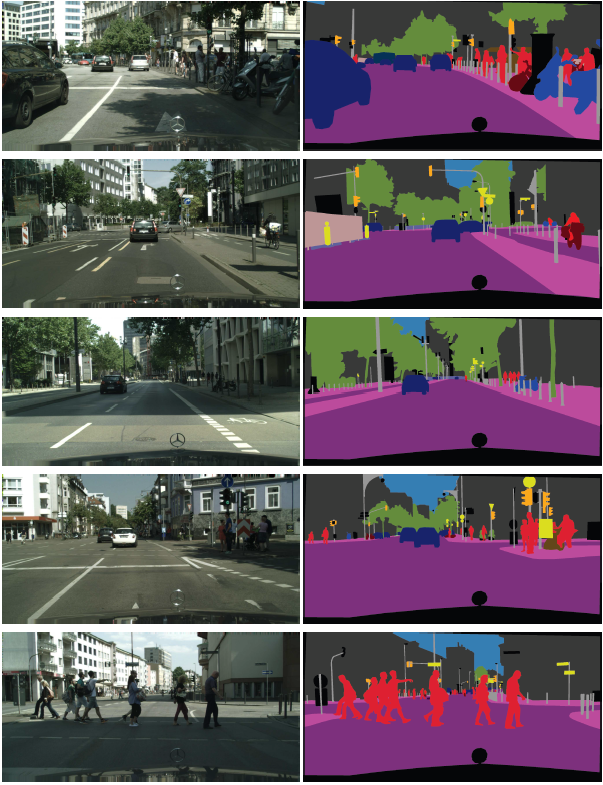
\includegraphics[width = \linewidth]{cityscapes4.png}
        \centering
        \caption{Esempio di immagini presenti in Cityscapes. A destra viene mostrata l'immagine originale mentre a sinistra la sua segmentazione semantica (Ground Truth).}
        \label{cityscapes}
    \end{figure} 
    ($512\times 256$, $1024\times 512$, $2048\times 1024$).
    \item {\bfseries{\emph{PASCAL Visual Object Classes (VOC)}}}\cite{VOC}: il seguente dataset 
    contiene più di 10.000 immagini con all'interno un totale di più di 20.000 
    oggetti raggruppati in 20 classi diverse (Fig. \ref{pascal}). Anche questo dataset, come 
    il precedente, viene utilizzato nella sezione di test per il task di 
    semantic segmentation in questo elaborato. Dettagliatamente, vengono 
    utilizzate delle sue immagini ridimensionate in formato $320\times 320$ e $512\times 320$.
    \begin{figure}
        \centering
        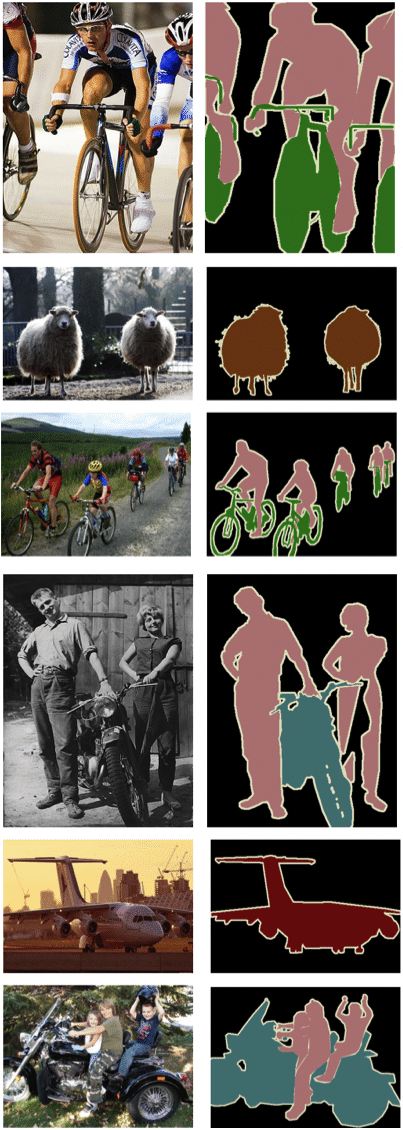
\includegraphics[width = 0.5\linewidth]{PascalVOC.png}
        \centering
        \caption{Esempio di immagini presenti in Pascal VOC. A destra viene mostrata l'immagine originale mentre a sinistra la sua segmentazione semantica (Ground Truth).}
        \label{pascal}
    \end{figure} 
    \item {\bfseries{\emph{MS Common Objects in Context (COCO)}}}\cite{COCO}: realizzato da 
    Microsoft, il dataset contiene più di 300.000 immagini di cui più di 
    200.000 sono etichettate (Fig. (\ref{MSCOCO_dataset})). Gli oggetti presenti sono più di 1.5 milioni e 
    sono raggruppati in 150 classi diverse. Principalmente questo dataset 
    viene utilizzato per attività di object detection, infatti ritorna utile 
    nella sezione di test successiva.
    \begin{figure}
        \centering
        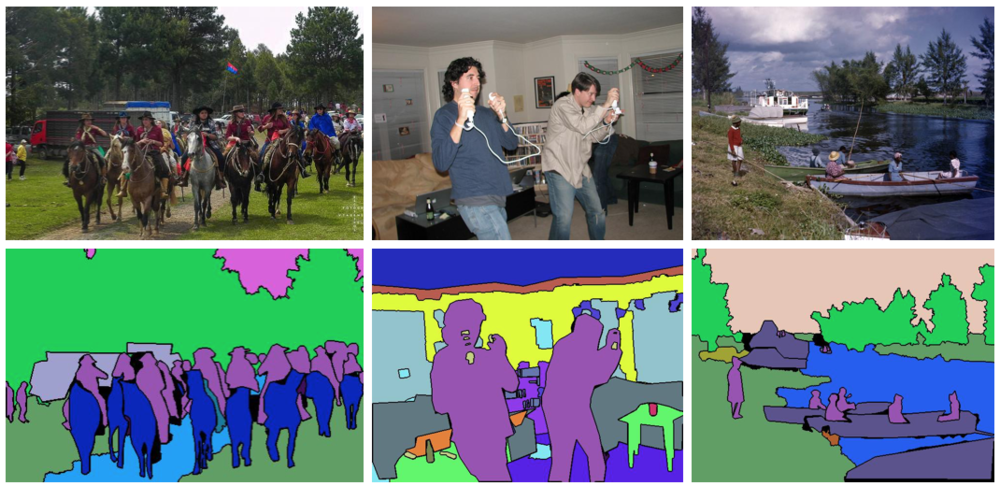
\includegraphics[width = \linewidth]{MSCOCO.png}
        \centering
        \caption{Esempio di immagini presenti in MS COCO. A destra viene mostrata l'immagine originale mentre a sinistra la sua segmentazione semantica (Ground Truth).}
        \label{MSCOCO_dataset}
    \end{figure} 
\end{itemize}

\newpage
\section{Test Performance}
Come brevemente accennato nel capitolo precedente, al fine di capire le 
potenzialità messe a disposizione dalle varie architetture di riferimento, di 
seguito viene riportato un test riguardante la comparazione dei \emph{Frame-per-
Second (FPS)} elaborati da ciascuna macchina. In ogni dataset esistono 
diversi set di immagini, ognuno con diversa risoluzione. Come inferenza, 
si è deciso di sottoporre in input i frame provenienti da sei diversi video 
(.mp4) e da due webcam, tutti aventi diversa risoluzione e numero di FPS (Tab. (\ref{source})).
Nelle tabelle seguenti, contenenti i valori ricavati dai test, sono presenti due tipologie di campi, maggiormente discussi nel capitolo precedente:
\begin{itemize}
    \item {\bfseries{\emph{Out}}}: indica il numero di FPS visualizzabili a schermo;
    \item {\bfseries{\emph{Net}}}: indica il numero di FPS elaborati da una specifica rete durante l'inferenza.
\end{itemize}

\begin{table}
    \renewcommand{\baselinestretch}{1}
    \centering
    \begin{adjustbox}{max width=\textwidth}
    \begin{tabular}{|c||c|c||}
        \hline
        \multirow{2}{*}{\bfseries{Sorgente}} & \multicolumn{2}{c||}{\bfseries{Specifiche Input}}\\            & \bfseries{Qualità} & \bfseries{FPS}\\
        \hline
        \hline
        \RN{1} Video & 240p & 60\\
        \hline
        \RN{2} Video & 360p & 30\\
        \hline 
        \RN{3} Video & 480p & 30\\
        \hline
        \RN{4} Video & 720p &  30\\
        \hline
        \RN{5} Video & 1080p & 30\\
        \hline
        \RN{6} Video & 1080p & 60\\
        \hline
        \RN{7} Webcam1 & 720p & 30\\
        \hline
        \RN{8} Webcam2 & 1080p & 30\\
        \hline
    \end{tabular}
    \end{adjustbox}
    \vspace{0.5cm}
    \caption{Specifiche sorgenti input.}
    \label{source}
\end{table}

\subsection{Test Performance Jetson Nano}
I test effettuati sulla scheda Jetson Nano sono stati eseguiti utilizzando due 
tipologie di librerie diverse, queste sono:
\begin{enumerate}
    \item {\bfseries{\emph{jetson.utils}}};
    \item {\bfseries{\emph{OpenCV}}}.
\end{enumerate}
Le prime sono librerie sviluppate interamente da NVidia che permettono 
l'ottimizzazione di sistemi embedded appartenenti alla famiglia Jetson. 
L'efficienza di questa libreria sta nell'utilizzo dell'SDK \emph{TensorRT} che offre 
una bassa latenza e un throughtput elevato per inferenze deep learning ad 
alte prestazioni. Tutte le applicazioni basate su TensorRT raggiungono 
delle prestazioni fino a 40 volte più veloci rispetto alle piattaforme dotate 
di sola CPU per l'inferenza. Solo le macchine provviste di schede grafiche 
NVidia possono avere questo beneficio in quanto su di esse vi è presente la 
tecnologia \emph{CUDA}, un modello di programmazione parallela che consente 
di ottimizzare l'inferenza grazie a librerie e strumenti di sviluppo basate 
su \emph{CUDA-X} per l'intelligenza artificiale, macchine a guida autonoma, 
elaborazioni ad alte prestazioni e grafica. Ritornando alle jetson.utils, 
queste mettono a disposizione dei modelli utili a compiere svariati compiti, 
come image recognition, object detection, semantic segmentation e pose estimation. 
I test svolti con queste librerie riguardano l'object detection (Tab.(\ref{obj_jetson_utils})) 
e la semantic segmentation (Tab.(\ref{sem_seg_jetson_utils})). A differenza della 
semantic segmentation, i testi per l'object detection vengono fatti su modelli 
pre-addestrati sulle immagine contenute nel dataset MS COCO avente 91 classi di 
elementi differenti. Per un dispositivo embedded di fascia economica, questi test 
raffigurano delle performance promettenti rispetto alla concorrenza.
I test effettuati con OpenCV invece vengono effettuati solo per il compito 
di semantic segmentation in quanto utilizzano file aventi formato \emph{ONNX}, 
messi a disposizione dalla community NVidia, che consentono l'interoperabilità 
tra i diversi framework AI con architetture sottostanti diverse. In poche 
parole, possiamo creare un modello già pre-addestrato e possiamo esportarlo 
in formato .ONNX ed eseguirlo su un'altra macchina con specifiche hardware 
differenti. Le performance ottenute con OpenCV per lo Jetson Nano sono 
visibili nella Tabella (\ref{sem_seg_jetson_utils_opencv_gpu}). Confrontando i 
risultati ottenuti con le jetson.utils, si evince che l'assenza di un 
ottimizzatore porta il sistema ad ottenere delle performance minori. 
Per comprendere le potenzialità offerte da modulo GPU, in Tab. 
(\ref{sem_seg_jetson_utils_opencv_cpu}) vengono riportate le performance 
ottenute dalla sua CPU. Per verificare la veridicità dei test effettuati, 
essendo questi effettuati solamente con le jetson.utils direttamente dal 
produttore della scheda embedded \cite{performance_obj_det_jetson}. Pertanto vengono 
riportati, nelle Tabelle (\ref{average performance jetson utils obj_det}) e (\ref{average performance jetson utils sem_seg}),  
i valori degli FPS medi, sia di Output che della Rete, per entrambe le 
frequenze di FPS in input. Quest'ultime riguardano le performance medie ottenute dall'uso delle jetson.utils, 
mentre quelle visibili nelle Tabelle (\ref{average performance jetson opencv GPU sem_seg}) e (\ref{average performance jetson opencv CPU sem_seg}) rappresentano le performance medie 
ottenute dall'uso delle OpenCV.
\begin{landscape}
    \renewcommand{\baselinestretch}{1}
    \centering
    \begin{table}
        \newarray\First
        \newarray\Second
        \newarray\Third
        \newarray\Fourth
        \newarray\Fifth
        \readarray{First}{16.82&34.48&16.12&33.88&18.6&34.96&18.04&34.05&17.46&33.74&15.6&34.47&11.54&34.78&11.88&34.72}
        \readarray{Second}{15.74&27.31&14.38&27.39&16.24&27.22&15.57&27.07&15.12&26.41&13.93&27&11&27.06&11.09&27.17}
        \readarray{Third}{13.77&21.55&12.38&22&13.93&21.69&13.81&21.67&13.83&21.51&12.31&21.56&9.82&21.81&9.78&21.71}
        \readarray{Fourth}{7.02&8.92&6.83&8.94&6.87&8.93&6.89&8.92&6.91&8.87&6.81&8.89&6.52&8.93&6.6&8.91}
        \readarray{Fifth}{7.02&9.13&6.79&9.12&7.02&9.16&6.96&9.15&6.92&9.07&6.76&9.15&6.57&9.08&6.61&9.08}
        {\scriptsize %
        \begin{tabular}{|c||c|c||c|c||c|c||c|c||c|c||c|c||c|c||c|c||}
            \hline
            & \multicolumn{16}{c||}{ \multirow{3}{*}{\bfseries{\large OBJECT DETECTION (DETECTNET) - JETSON NANO (utils)}}}\\
            & \multicolumn{16}{c||}{}\\
            & \multicolumn{16}{c||}{}\\
            \hline
            \multirow{2}{*}{\bfseries{\large Modelli}} 
            & \multicolumn{2}{c||}{\bfseries{\normalsize Webcam1}} & \multicolumn{2}{c||}{\bfseries{\normalsize Webcam2}} & \multicolumn{2}{c||}{\bfseries{\normalsize \RN{1} Video}} & \multicolumn{2}{c||}{\bfseries{\normalsize \RN{2} Video}} & \multicolumn{2}{c||}{\bfseries{\normalsize \RN{3} Video}} & \multicolumn{2}{c||}{\bfseries{\normalsize \RN{4} Video}} & \multicolumn{2}{c||}{\bfseries{\normalsize \RN{5} Video}} & \multicolumn{2}{c||}{\bfseries{\normalsize \RN{6} Video}}\\            & \bfseries{\footnotesize Out} & \bfseries{\footnotesize Net} & \bfseries{\footnotesize Out} & \bfseries{\footnotesize Net} & \bfseries{\footnotesize Out} & \bfseries{\footnotesize Net} & \bfseries{\footnotesize Out} & \bfseries{\footnotesize Net} & \bfseries{\footnotesize Out} & \bfseries{\footnotesize Net} & \bfseries{\footnotesize Out} & \bfseries{\footnotesize Net} & \bfseries{\footnotesize Out} & \bfseries{\footnotesize Net} & \bfseries{\footnotesize Out} & \bfseries{\footnotesize Net}\\
            \hline
            \multirow{2}{*}{SSD-MOBILENET-V1} & \multirow{2}{*}{\First(1)} & \multirow{2}{*}{\First(2)} & \multirow{2}{*}{\First(3)} & \multirow{2}{*}{\First(4)} & \multirow{2}{*}{\First(5)} & \multirow{2}{*}{\First(6)} & \multirow{2}{*}{\First(7)} & \multirow{2}{*}{\First(8)} & \multirow{2}{*}{\First(9)} & \multirow{2}{*}{\First(10)} & \multirow{2}{*}{\First(11)} & \multirow{2}{*}{\First(12)} & \multirow{2}{*}{\First(13)} & \multirow{2}{*}{\First(14)} & \multirow{2}{*}{\First(15)} & \multirow{2}{*}{\First(16)}\\
            & & & & & & & & & & & & & & & &\\
            \hline
            \multirow{2}{*}{SSD-MOBILENET-V2}& \multirow{2}{*}{\Second(1)} & \multirow{2}{*}{\Second(2)} & \multirow{2}{*}{\Second(3)} & \multirow{2}{*}{\Second(4)} & \multirow{2}{*}{\Second(5)} & \multirow{2}{*}{\Second(6)} & \multirow{2}{*}{\Second(7)} & \multirow{2}{*}{\Second(8)} & \multirow{2}{*}{\Second(9)} & \multirow{2}{*}{\Second(10)} & \multirow{2}{*}{\Second(11)} & \multirow{2}{*}{\Second(12)} & \multirow{2}{*}{\Second(13)} & \multirow{2}{*}{\Second(14)} & \multirow{2}{*}{\Second(15)} & \multirow{2}{*}{\Second(16)}\\
            & & & & & & & & & & & & & & & &\\
            \hline 
            \multirow{2}{*}{SSD-INCEPTION-V2}& \multirow{2}{*}{\Third(1)} & \multirow{2}{*}{\Third(2)} & \multirow{2}{*}{\Third(3)} & \multirow{2}{*}{\Third(4)} & \multirow{2}{*}{\Third(5)} & \multirow{2}{*}{\Third(6)} & \multirow{2}{*}{\Third(7)} & \multirow{2}{*}{\Third(8)} & \multirow{2}{*}{\Third(9)} & \multirow{2}{*}{\Third(10)} & \multirow{2}{*}{\Third(11)} & \multirow{2}{*}{\Third(12)} & \multirow{2}{*}{\Third(13)} & \multirow{2}{*}{\Third(14)} & \multirow{2}{*}{\Third(15)} & \multirow{2}{*}{\Third(16)}\\
            & & & & & & & & & & & & & & & &\\
            \hline
            \multirow{2}{*}{PEDNET}& \multirow{2}{*}{\Fourth(1)} & \multirow{2}{*}{\Fourth(2)} & \multirow{2}{*}{\Fourth(3)} & \multirow{2}{*}{\Fourth(4)} & \multirow{2}{*}{\Fourth(5)} & \multirow{2}{*}{\Fourth(6)} & \multirow{2}{*}{\Fourth(7)} & \multirow{2}{*}{\Fourth(8)} & \multirow{2}{*}{\Fourth(9)} & \multirow{2}{*}{\Fourth(10)} & \multirow{2}{*}{\Fourth(11)} & \multirow{2}{*}{\Fourth(12)} & \multirow{2}{*}{\Fourth(13)} & \multirow{2}{*}{\Fourth(14)} & \multirow{2}{*}{\Fourth(15)} & \multirow{2}{*}{\Fourth(16)}\\
            & & & & & & & & & & & & & & & &\\
            \hline
            \multirow{2}{*}{MULTIPEDNET}& \multirow{2}{*}{\Fifth(1)} & \multirow{2}{*}{\Fifth(2)} & \multirow{2}{*}{\Fifth(3)} & \multirow{2}{*}{\Fifth(4)} & \multirow{2}{*}{\Fifth(5)} & \multirow{2}{*}{\Fifth(6)} & \multirow{2}{*}{\Fifth(7)} & \multirow{2}{*}{\Fifth(8)} & \multirow{2}{*}{\Fifth(9)} & \multirow{2}{*}{\Fifth(10)} & \multirow{2}{*}{\Fifth(11)} & \multirow{2}{*}{\Fifth(12)} & \multirow{2}{*}{\Fifth(13)} & \multirow{2}{*}{\Fifth(14)} & \multirow{2}{*}{\Fifth(15)} & \multirow{2}{*}{\Fifth(16)}\\
            & & & & & & & & & & & & & & & &\\
            \hline
        \end{tabular}
        }%
        \vspace{0.2cm}
        \caption{FPS Performance nell'attività di Object Detection su Jetson Nano (\emph{utils}).}
        \label{obj_jetson_utils}
    \end{table}

    \begin{table}
        \newarray\Firsts
        \newarray\Second
        \newarray\Third
        \newarray\Fourth
        \newarray\Fifth
        \readarray{Firsts}{8.25&48.12&8.37&48.94&20.49&48.92&16.68&48.75&15.7&48.6&9.19&48.24&4.43&48.42&4.63&48.08}
        \readarray{Second}{5.76&12.27&5.57&12.35&8.22&12.34&7.38&12.27&7.46&12.34&5.46&12.3&4.43&12.21&3.96&12.31}
        \readarray{Third}{3.79&3.04&2.56&3.06&4.41&3.06&2.38&3.06&4.31&3.06&2.17&3.06&3.58&3.06&1.79&3.02}
        \readarray{Fourth}{8.96&46.06&7.9&46.44&20.19&46.43&16.37&46.46&15.32&46.63&7.82&46.26&4.78&46.03&4.96&45.98}
        \readarray{Fifth}{8.4&34.31&8.15&34.92&17.15&34.35&13.52&34.26&13.82&34.43&7.42&34.21&4.5&34.61&4.74&34.44}
        {\scriptsize %
        \begin{tabular}{|c||c|c||c|c||c|c||c|c||c|c||c|c||c|c||c|c||}
            \hline
            & \multicolumn{16}{c||}{ \multirow{3}{*}{\bfseries{\large SEMANTIC SEGMENTATION (SEGNET) - JETSON NANO (utils)}}}\\
            & \multicolumn{16}{c||}{}\\
            & \multicolumn{16}{c||}{}\\
            \hline
            \multirow{2}{*}{\bfseries{\large Modelli-Dati}} 
            & \multicolumn{2}{c||}{\bfseries{\normalsize Webcam1}} & \multicolumn{2}{c||}{\bfseries{\normalsize Webcam2}} & \multicolumn{2}{c||}{\bfseries{\normalsize \RN{1} Video}} & \multicolumn{2}{c||}{\bfseries{\normalsize \RN{2} Video}} & \multicolumn{2}{c||}{\bfseries{\normalsize \RN{3} Video}} & \multicolumn{2}{c||}{\bfseries{\normalsize \RN{4} Video}} & \multicolumn{2}{c||}{\bfseries{\normalsize \RN{5} Video}} & \multicolumn{2}{c||}{\bfseries{\normalsize \RN{6} Video}}\\            & \bfseries{\footnotesize Out} & \bfseries{\footnotesize Net} & \bfseries{\footnotesize Out} & \bfseries{\footnotesize Net} & \bfseries{\footnotesize Out} & \bfseries{\footnotesize Net} & \bfseries{\footnotesize Out} & \bfseries{\footnotesize Net} & \bfseries{\footnotesize Out} & \bfseries{\footnotesize Net} & \bfseries{\footnotesize Out} & \bfseries{\footnotesize Net} & \bfseries{\footnotesize Out} & \bfseries{\footnotesize Net} & \bfseries{\footnotesize Out} & \bfseries{\footnotesize Net}\\
            \hline
            \multirow{2}{*}{RN18-CS (512x256)} & \multirow{2}{*}{\Firsts(1)} & \multirow{2}{*}{\Firsts(2)} & \multirow{2}{*}{\Firsts(3)} & \multirow{2}{*}{\Firsts(4)} & \multirow{2}{*}{\Firsts(5)} & \multirow{2}{*}{\Firsts(6)} & \multirow{2}{*}{\Firsts(7)} & \multirow{2}{*}{\Firsts(8)} & \multirow{2}{*}{\Firsts(9)} & \multirow{2}{*}{\Firsts(10)} & \multirow{2}{*}{\Firsts(11)} & \multirow{2}{*}{\Firsts(12)} & \multirow{2}{*}{\Firsts(13)} & \multirow{2}{*}{\Firsts(14)} & \multirow{2}{*}{\Firsts(15)} & \multirow{2}{*}{\Firsts(16)}\\
            & & & & & & & & & & & & & & & &\\
            \hline
            \multirow{2}{*}{RN18-CS (1024x512)}& \multirow{2}{*}{\Second(1)} & \multirow{2}{*}{\Second(2)} & \multirow{2}{*}{\Second(3)} & \multirow{2}{*}{\Second(4)} & \multirow{2}{*}{\Second(5)} & \multirow{2}{*}{\Second(6)} & \multirow{2}{*}{\Second(7)} & \multirow{2}{*}{\Second(8)} & \multirow{2}{*}{\Second(9)} & \multirow{2}{*}{\Second(10)} & \multirow{2}{*}{\Second(11)} & \multirow{2}{*}{\Second(12)} & \multirow{2}{*}{\Second(13)} & \multirow{2}{*}{\Second(14)} & \multirow{2}{*}{\Second(15)} & \multirow{2}{*}{\Second(16)}\\
            & & & & & & & & & & & & & & & &\\
            \hline 
            \multirow{2}{*}{RN18-CS (2048x1024)}& \multirow{2}{*}{\Third(1)} & \multirow{2}{*}{\Third(2)} & \multirow{2}{*}{\Third(3)} & \multirow{2}{*}{\Third(4)} & \multirow{2}{*}{\Third(5)} & \multirow{2}{*}{\Third(6)} & \multirow{2}{*}{\Third(7)} & \multirow{2}{*}{\Third(8)} & \multirow{2}{*}{\Third(9)} & \multirow{2}{*}{\Third(10)} & \multirow{2}{*}{\Third(11)} & \multirow{2}{*}{\Third(12)} & \multirow{2}{*}{\Third(13)} & \multirow{2}{*}{\Third(14)} & \multirow{2}{*}{\Third(15)} & \multirow{2}{*}{\Third(16)}\\
            & & & & & & & & & & & & & & & &\\
            \hline
            \multirow{2}{*}{RN18-VOC (320x320)}& \multirow{2}{*}{\Fourth(1)} & \multirow{2}{*}{\Fourth(2)} & \multirow{2}{*}{\Fourth(3)} & \multirow{2}{*}{\Fourth(4)} & \multirow{2}{*}{\Fourth(5)} & \multirow{2}{*}{\Fourth(6)} & \multirow{2}{*}{\Fourth(7)} & \multirow{2}{*}{\Fourth(8)} & \multirow{2}{*}{\Fourth(9)} & \multirow{2}{*}{\Fourth(10)} & \multirow{2}{*}{\Fourth(11)} & \multirow{2}{*}{\Fourth(12)} & \multirow{2}{*}{\Fourth(13)} & \multirow{2}{*}{\Fourth(14)} & \multirow{2}{*}{\Fourth(15)} & \multirow{2}{*}{\Fourth(16)}\\
            & & & & & & & & & & & & & & & &\\
            \hline
            \multirow{2}{*}{RN18-VOC (512x320)}& \multirow{2}{*}{\Fifth(1)} & \multirow{2}{*}{\Fifth(2)} & \multirow{2}{*}{\Fifth(3)} & \multirow{2}{*}{\Fifth(4)} & \multirow{2}{*}{\Fifth(5)} & \multirow{2}{*}{\Fifth(6)} & \multirow{2}{*}{\Fifth(7)} & \multirow{2}{*}{\Fifth(8)} & \multirow{2}{*}{\Fifth(9)} & \multirow{2}{*}{\Fifth(10)} & \multirow{2}{*}{\Fifth(11)} & \multirow{2}{*}{\Fifth(12)} & \multirow{2}{*}{\Fifth(13)} & \multirow{2}{*}{\Fifth(14)} & \multirow{2}{*}{\Fifth(15)} & \multirow{2}{*}{\Fifth(16)}\\
            & & & & & & & & & & & & & & & &\\
            \hline
        \end{tabular}
        }%
        \vspace{0.2cm}
        \caption{FPS Performance nell'attività di Semantic Segmentation su Jetson Nano (\emph{utils}).}
        \label{sem_seg_jetson_utils}
    \end{table}
\end{landscape}

\begin{landscape}
    \renewcommand{\baselinestretch}{1}
    \centering
    \begin{table}
        \newarray\Firsts
        \newarray\Second
        \newarray\Third
        \newarray\Fourth
        \newarray\Fifth
        \readarray{Firsts}{6.19&18.93&2&19.63&16.41&19.81&14.27&19.69&14.24&19.7&6.62&19.53&4.88&19.24&4.91&19.35}
        \readarray{Second}{3.4&4.99&2&5.53&5.02&5.39&4.75&5.2&4.76&5.2&3.38&4.77&2.86&4.99&2.86&5.36}
        \readarray{Third}{1.09&1.44&1.24&1.45&1.34&1.46&1.34&1.46&1.31&1.46&1.23&1.45&1&1.46&1&1.46}
        \readarray{Fourth}{6.02&17.12&2&17.79&15.41&17.91&13.46&17.76&13.43&17.6&6.56&17.6&4.42&17.33&4.81&17.5}
        \readarray{Fifth}{5.91&14.6&2&14.97&12.9&15.08&11.51&15&11.51&14.98&5.93&14.9&4.51&14.77&4.51&14.85}
        \centering
        {\scriptsize %
        \begin{tabular}{|c||c|c||c|c||c|c||c|c||c|c||c|c||c|c||c|c||}
            \hline
            & \multicolumn{16}{c||}{ \multirow{3}{*}{\bfseries{\large SEMANTIC SEGMENTATION - JETSON NANO (OPENCV - GPU)}}}\\
            & \multicolumn{16}{c||}{}\\
            & \multicolumn{16}{c||}{}\\
            \hline
            \multirow{2}{*}{\bfseries{\large Modelli-Dati}} 
            & \multicolumn{2}{c||}{\bfseries{\normalsize Webcam1}} & \multicolumn{2}{c||}{\bfseries{\normalsize Webcam2}} & \multicolumn{2}{c||}{\bfseries{\normalsize \RN{1} Video}} & \multicolumn{2}{c||}{\bfseries{\normalsize \RN{2} Video}} & \multicolumn{2}{c||}{\bfseries{\normalsize \RN{3} Video}} & \multicolumn{2}{c||}{\bfseries{\normalsize \RN{4} Video}} & \multicolumn{2}{c||}{\bfseries{\normalsize \RN{5} Video}} & \multicolumn{2}{c||}{\bfseries{\normalsize \RN{6} Video}}\\            & \bfseries{\footnotesize Out} & \bfseries{\footnotesize Net} & \bfseries{\footnotesize Out} & \bfseries{\footnotesize Net} & \bfseries{\footnotesize Out} & \bfseries{\footnotesize Net} & \bfseries{\footnotesize Out} & \bfseries{\footnotesize Net} & \bfseries{\footnotesize Out} & \bfseries{\footnotesize Net} & \bfseries{\footnotesize Out} & \bfseries{\footnotesize Net} & \bfseries{\footnotesize Out} & \bfseries{\footnotesize Net} & \bfseries{\footnotesize Out} & \bfseries{\footnotesize Net}\\
            \hline
            \multirow{2}{*}{RN18-CS (512x256)} & \multirow{2}{*}{\Firsts(1)} & \multirow{2}{*}{\Firsts(2)} & \multirow{2}{*}{\Firsts(3)} & \multirow{2}{*}{\Firsts(4)} & \multirow{2}{*}{\Firsts(5)} & \multirow{2}{*}{\Firsts(6)} & \multirow{2}{*}{\Firsts(7)} & \multirow{2}{*}{\Firsts(8)} & \multirow{2}{*}{\Firsts(9)} & \multirow{2}{*}{\Firsts(10)} & \multirow{2}{*}{\Firsts(11)} & \multirow{2}{*}{\Firsts(12)} & \multirow{2}{*}{\Firsts(13)} & \multirow{2}{*}{\Firsts(14)} & \multirow{2}{*}{\Firsts(15)} & \multirow{2}{*}{\Firsts(16)}\\
            & & & & & & & & & & & & & & & &\\
            \hline
            \multirow{2}{*}{RN18-CS (1024x512)}& \multirow{2}{*}{\Second(1)} & \multirow{2}{*}{\Second(2)} & \multirow{2}{*}{\Second(3)} & \multirow{2}{*}{\Second(4)} & \multirow{2}{*}{\Second(5)} & \multirow{2}{*}{\Second(6)} & \multirow{2}{*}{\Second(7)} & \multirow{2}{*}{\Second(8)} & \multirow{2}{*}{\Second(9)} & \multirow{2}{*}{\Second(10)} & \multirow{2}{*}{\Second(11)} & \multirow{2}{*}{\Second(12)} & \multirow{2}{*}{\Second(13)} & \multirow{2}{*}{\Second(14)} & \multirow{2}{*}{\Second(15)} & \multirow{2}{*}{\Second(16)}\\
            & & & & & & & & & & & & & & & &\\
            \hline 
            \multirow{2}{*}{RN18-CS (2048x1024)}& \multirow{2}{*}{\Third(1)} & \multirow{2}{*}{\Third(2)} & \multirow{2}{*}{\Third(3)} & \multirow{2}{*}{\Third(4)} & \multirow{2}{*}{\Third(5)} & \multirow{2}{*}{\Third(6)} & \multirow{2}{*}{\Third(7)} & \multirow{2}{*}{\Third(8)} & \multirow{2}{*}{\Third(9)} & \multirow{2}{*}{\Third(10)} & \multirow{2}{*}{\Third(11)} & \multirow{2}{*}{\Third(12)} & \multirow{2}{*}{\Third(13)} & \multirow{2}{*}{\Third(14)} & \multirow{2}{*}{\Third(15)} & \multirow{2}{*}{\Third(16)}\\
            & & & & & & & & & & & & & & & &\\
            \hline
            \multirow{2}{*}{RN18-VOC (320x320)}& \multirow{2}{*}{\Fourth(1)} & \multirow{2}{*}{\Fourth(2)} & \multirow{2}{*}{\Fourth(3)} & \multirow{2}{*}{\Fourth(4)} & \multirow{2}{*}{\Fourth(5)} & \multirow{2}{*}{\Fourth(6)} & \multirow{2}{*}{\Fourth(7)} & \multirow{2}{*}{\Fourth(8)} & \multirow{2}{*}{\Fourth(9)} & \multirow{2}{*}{\Fourth(10)} & \multirow{2}{*}{\Fourth(11)} & \multirow{2}{*}{\Fourth(12)} & \multirow{2}{*}{\Fourth(13)} & \multirow{2}{*}{\Fourth(14)} & \multirow{2}{*}{\Fourth(15)} & \multirow{2}{*}{\Fourth(16)}\\
            & & & & & & & & & & & & & & & &\\
            \hline
            \multirow{2}{*}{RN18-VOC (512x320)}& \multirow{2}{*}{\Fifth(1)} & \multirow{2}{*}{\Fifth(2)} & \multirow{2}{*}{\Fifth(3)} & \multirow{2}{*}{\Fifth(4)} & \multirow{2}{*}{\Fifth(5)} & \multirow{2}{*}{\Fifth(6)} & \multirow{2}{*}{\Fifth(7)} & \multirow{2}{*}{\Fifth(8)} & \multirow{2}{*}{\Fifth(9)} & \multirow{2}{*}{\Fifth(10)} & \multirow{2}{*}{\Fifth(11)} & \multirow{2}{*}{\Fifth(12)} & \multirow{2}{*}{\Fifth(13)} & \multirow{2}{*}{\Fifth(14)} & \multirow{2}{*}{\Fifth(15)} & \multirow{2}{*}{\Fifth(16)}\\
            & & & & & & & & & & & & & & & &\\
            \hline
        \end{tabular}
        }%
        \vspace{0.2cm}
        \caption{FPS performance nell'attività di Semantic Segmentation su Jetson Nano (\emph{OpenCV - GPU})}
        \label{sem_seg_jetson_utils_opencv_gpu}
    \end{table}

    \begin{table}
        \newarray\Firsts
        \newarray\Second
        \newarray\Third
        \newarray\Fourth
        \newarray\Fifth
        \readarray{Firsts}{1.31&1.48&1.33&1.47&1.68&1.68&1.69&1.74&1.66&1.71&1.51&1.7&1.3&1.59&1.3&1.59}
        \readarray{Second}{0.35&36&0.35&0.36&0.4&0.4&0.41&0.41&0.4&0.4&0.39&0.41&0.37&0.39&0.38&0.4}
        \readarray{Third}{0.09&0.069&0.08&0.08&0.09&0.09&0.1&0.1&0.1&0.1&0.1&0.1&0.09&0.1&0.09&0.1}
        \readarray{Fourth}{1.63&1.88&1.71&1.92&2.18&2.2&2.15&2.22&2.14&2.22&1.88&2.15&1.6&2.06&1.6&2.08}
        \readarray{Fifth}{1.1&1.22&1.11&1.21&1.39&1.39&1.38&1.42&1.37&1.4&1.26&1.38&1.12&1.33&1.12&1.33}
        \centering
        {\scriptsize %
        \begin{tabular}{|c||c|c||c|c||c|c||c|c||c|c||c|c||c|c||c|c||}
            \hline
            & \multicolumn{16}{c||}{ \multirow{3}{*}{\bfseries{\large SEMANTIC SEGMENTATION - JETSON NANO (OPENCV - CPU)}}}\\
            & \multicolumn{16}{c||}{}\\
            & \multicolumn{16}{c||}{}\\
            \hline
            \multirow{2}{*}{\bfseries{\large Modelli-Dati}} 
            & \multicolumn{2}{c||}{\bfseries{\normalsize Webcam1}} & \multicolumn{2}{c||}{\bfseries{\normalsize Webcam2}} & \multicolumn{2}{c||}{\bfseries{\normalsize \RN{1} Video}} & \multicolumn{2}{c||}{\bfseries{\normalsize \RN{2} Video}} & \multicolumn{2}{c||}{\bfseries{\normalsize \RN{3} Video}} & \multicolumn{2}{c||}{\bfseries{\normalsize \RN{4} Video}} & \multicolumn{2}{c||}{\bfseries{\normalsize \RN{5} Video}} & \multicolumn{2}{c||}{\bfseries{\normalsize \RN{6} Video}}\\            & \bfseries{\footnotesize Out} & \bfseries{\footnotesize Net} & \bfseries{\footnotesize Out} & \bfseries{\footnotesize Net} & \bfseries{\footnotesize Out} & \bfseries{\footnotesize Net} & \bfseries{\footnotesize Out} & \bfseries{\footnotesize Net} & \bfseries{\footnotesize Out} & \bfseries{\footnotesize Net} & \bfseries{\footnotesize Out} & \bfseries{\footnotesize Net} & \bfseries{\footnotesize Out} & \bfseries{\footnotesize Net} & \bfseries{\footnotesize Out} & \bfseries{\footnotesize Net}\\
            \hline
            \multirow{2}{*}{RN18-CS (512x256)} & \multirow{2}{*}{\Firsts(1)} & \multirow{2}{*}{\Firsts(2)} & \multirow{2}{*}{\Firsts(3)} & \multirow{2}{*}{\Firsts(4)} & \multirow{2}{*}{\Firsts(5)} & \multirow{2}{*}{\Firsts(6)} & \multirow{2}{*}{\Firsts(7)} & \multirow{2}{*}{\Firsts(8)} & \multirow{2}{*}{\Firsts(9)} & \multirow{2}{*}{\Firsts(10)} & \multirow{2}{*}{\Firsts(11)} & \multirow{2}{*}{\Firsts(12)} & \multirow{2}{*}{\Firsts(13)} & \multirow{2}{*}{\Firsts(14)} & \multirow{2}{*}{\Firsts(15)} & \multirow{2}{*}{\Firsts(16)}\\
            & & & & & & & & & & & & & & & &\\
            \hline
            \multirow{2}{*}{RN18-CS (1024x512)}& \multirow{2}{*}{\Second(1)} & \multirow{2}{*}{\Second(2)} & \multirow{2}{*}{\Second(3)} & \multirow{2}{*}{\Second(4)} & \multirow{2}{*}{\Second(5)} & \multirow{2}{*}{\Second(6)} & \multirow{2}{*}{\Second(7)} & \multirow{2}{*}{\Second(8)} & \multirow{2}{*}{\Second(9)} & \multirow{2}{*}{\Second(10)} & \multirow{2}{*}{\Second(11)} & \multirow{2}{*}{\Second(12)} & \multirow{2}{*}{\Second(13)} & \multirow{2}{*}{\Second(14)} & \multirow{2}{*}{\Second(15)} & \multirow{2}{*}{\Second(16)}\\
            & & & & & & & & & & & & & & & &\\
            \hline 
            \multirow{2}{*}{RN18-CS (2048x1024)}& \multirow{2}{*}{\Third(1)} & \multirow{2}{*}{\Third(2)} & \multirow{2}{*}{\Third(3)} & \multirow{2}{*}{\Third(4)} & \multirow{2}{*}{\Third(5)} & \multirow{2}{*}{\Third(6)} & \multirow{2}{*}{\Third(7)} & \multirow{2}{*}{\Third(8)} & \multirow{2}{*}{\Third(9)} & \multirow{2}{*}{\Third(10)} & \multirow{2}{*}{\Third(11)} & \multirow{2}{*}{\Third(12)} & \multirow{2}{*}{\Third(13)} & \multirow{2}{*}{\Third(14)} & \multirow{2}{*}{\Third(15)} & \multirow{2}{*}{\Third(16)}\\
            & & & & & & & & & & & & & & & &\\
            \hline
            \multirow{2}{*}{RN18-VOC (320x320)}& \multirow{2}{*}{\Fourth(1)} & \multirow{2}{*}{\Fourth(2)} & \multirow{2}{*}{\Fourth(3)} & \multirow{2}{*}{\Fourth(4)} & \multirow{2}{*}{\Fourth(5)} & \multirow{2}{*}{\Fourth(6)} & \multirow{2}{*}{\Fourth(7)} & \multirow{2}{*}{\Fourth(8)} & \multirow{2}{*}{\Fourth(9)} & \multirow{2}{*}{\Fourth(10)} & \multirow{2}{*}{\Fourth(11)} & \multirow{2}{*}{\Fourth(12)} & \multirow{2}{*}{\Fourth(13)} & \multirow{2}{*}{\Fourth(14)} & \multirow{2}{*}{\Fourth(15)} & \multirow{2}{*}{\Fourth(16)}\\
            & & & & & & & & & & & & & & & &\\
            \hline
            \multirow{2}{*}{RN18-VOC (512x320)}& \multirow{2}{*}{\Fifth(1)} & \multirow{2}{*}{\Fifth(2)} & \multirow{2}{*}{\Fifth(3)} & \multirow{2}{*}{\Fifth(4)} & \multirow{2}{*}{\Fifth(5)} & \multirow{2}{*}{\Fifth(6)} & \multirow{2}{*}{\Fifth(7)} & \multirow{2}{*}{\Fifth(8)} & \multirow{2}{*}{\Fifth(9)} & \multirow{2}{*}{\Fifth(10)} & \multirow{2}{*}{\Fifth(11)} & \multirow{2}{*}{\Fifth(12)} & \multirow{2}{*}{\Fifth(13)} & \multirow{2}{*}{\Fifth(14)} & \multirow{2}{*}{\Fifth(15)} & \multirow{2}{*}{\Fifth(16)}\\
            & & & & & & & & & & & & & & & &\\
            \hline
        \end{tabular}
        }%
        \vspace{0.2cm}
        \caption{FPS performance nell'attività di Semantic Segmentation su Jetson Nano (\emph{OpenCV - CPU})}
        \label{sem_seg_jetson_utils_opencv_cpu}
    \end{table}
\end{landscape}

\begin{table}
    \renewcommand{\baselinestretch}{1}
    \centering
    \begin{adjustbox}{max width=\textwidth}
    \begin{tabular}{|c||c|c||c|c||}
        \hline
        \multirow{2}{*}{\bfseries{\Large Modelli}} & \multicolumn{2}{c||}{\bfseries{30 FPS}} & \multicolumn{2}{c||}{\bfseries{60 FPS}}\\            & \bfseries{Output} & \bfseries{Network} & \bfseries{Output} & \bfseries{Network}\\
        \hline
        \hline
        SSD-MOBILENET-V1 & 15.93 & 34.23 & 15.24 & 34.84\\
        \hline
        SSD-MOBILENET-V2 & 14.29 & 27.04 & 13,66 & 27.19\\
        \hline 
        SSD-INCEPTION-V2 & 12.65 & 21.68 & 11.85 & 21.7\\
        \hline
        PEDNET & 6.83 &  8.91 & 6.73 & 8.92\\
        \hline
        MULTIPEDNET & 6.84 & 9.11 & 6.81 & 9.12\\
        \hline
    \end{tabular}
    \end{adjustbox}
    \vspace{0.5cm}
    \caption{Performance FPS medi nell'attività di Object Detection su Jetson Nano (\emph{utils}).}
    \label{average performance jetson utils obj_det}
\end{table}

\begin{table}
    \renewcommand{\baselinestretch}{1}
    \centering
    \begin{adjustbox}{max width=\textwidth}
    \begin{tabular}{|c||c|c||c|c||}
        \hline
        \multirow{2}{*}{\bfseries{\Large Modelli-Dataset}} & \multicolumn{2}{c||}{\bfseries{30 FPS}} & \multicolumn{2}{c||}{\bfseries{60 FPS}}\\            & \bfseries{Output} & \bfseries{Network} & \bfseries{Output} & \bfseries{Network}\\
        \hline
        \hline
        RN18-CS (512x256) & 10.43 & 48.51 & 12.56 & 48.5\\
        \hline
        RN18-CS (1024x512) & 6.01 & 12.29 & 6.09 & 12.32\\
        \hline 
        RN18-CS (2048x1024) & 3,13 & 3,05 & 3.1 & 3.04\\
        \hline
        RN18-VOC (320x320) & 10.19 &  46.31 & 12.57 & 46.20\\
        \hline
        RN18-VOC (512x320) & 9.30 & 34.45 & 10.94 & 34.39\\
        \hline
    \end{tabular}
    \end{adjustbox}
    \vspace{0.5cm}
    \caption{Performance FPS medi nell'attività di Semantic Segmentation Jetson Nano (\emph{utils}).}
    \label{average performance jetson utils sem_seg}
\end{table}

\begin{table}
    \renewcommand{\baselinestretch}{1}
    \centering
    \begin{adjustbox}{max width=\textwidth}
    \begin{tabular}{|c||c|c||c|c||}
        \hline
        \multirow{2}{*}{\bfseries{\Large Modelli-Dataset}} & \multicolumn{2}{c||}{\bfseries{30 FPS}} & \multicolumn{2}{c||}{\bfseries{60 FPS}}\\            & \bfseries{Output} & \bfseries{Network} & \bfseries{Output} & \bfseries{Network}\\
        \hline
        \hline
        RN18-CS (512x256) & 8.03 & 19.45 & 10.66 & 19.58\\
        \hline
        RN18-CS (1024x512) & 3.52 & 5.11 & 3.94 & 5.37\\
        \hline 
        RN18-CS (2048x1024) & 1.20 & 1.45 & 1,17 & 1.46\\
        \hline
        RN18-VOC (320x320) & 7.68 &  17.53 & 10.11 & 17.7\\
        \hline
        RN18-VOC (512x320) & 6.89 & 14.87 & 8.7 & 14.96\\
        \hline
    \end{tabular}
    \end{adjustbox}
    \vspace{0.5cm}
    \caption{Performance FPS medi nell'attività di Semantic Segmentation Jetson Nano (\emph{OpenCV - GPU}).}
    \label{average performance jetson opencv GPU sem_seg}
\end{table}

\begin{table}
    \renewcommand{\baselinestretch}{1}
    \centering
    \begin{adjustbox}{max width=\textwidth}
    \begin{tabular}{|c||c|c||c|c||}
        \hline
        \multirow{2}{*}{\bfseries{\Large Modelli-Dataset}} & \multicolumn{2}{c||}{\bfseries{30 FPS}} & \multicolumn{2}{c||}{\bfseries{60 FPS}}\\            & \bfseries{Output} & \bfseries{Network} & \bfseries{Output} & \bfseries{Network}\\
        \hline
        \hline
        RN18-CS (512x256) & 1.46 & 1.61 & 1.49 & 1.63\\
        \hline
        RN18-CS (1024x512) & 0.37 & 0.38 & 0.39 & 0.4\\
        \hline 
        RN18-CS (2048x1024) & 0.09 & 0.09 & 0.09 & 0.09\\
        \hline
        RN18-VOC (320x320) & 1.85 &  2.07 & 1.89 & 2.14\\
        \hline
        RN18-VOC (512x320) & 1.22 & 1.32 & 1.25 & 1.36\\
        \hline
    \end{tabular}
    \end{adjustbox}
    \vspace{0.5cm}
    \caption{Performance FPS medi nell'attività di Semantic Segmentation Jetson Nano (\emph{OpenCV - CPU}).}
    \label{average performance jetson opencv CPU sem_seg}
\end{table}

\newpage
\subsection{Test Performance Computer}
Non disponendo di una scheda grafica NVidia, sul computer di riferimento i 
test vengono effettuati utilizzando solo la sua CPU utilizzando quindi la sola 
libreria OpenCV. I test sono riportati nella Tabella (\ref{sem_seg_perf_comp}). Comparando 
i risultati ottenuti con quelli dello Jetson Nano, i test mostrano come 
un tale dispositivo, di fascia economica e prestazioni alte, ottenga delle 
performance migliori. Le considerazioni cambiano quando la comparazione 
avviene tra le performance ottenute dalle jetson.utils e quelle del PC. In 
quest'ultimo caso si evidenziano le vere potenzialità dello Jetson Nano. Pur 
avendo una potenza computazionale di gran lunga minore rispetto a quella 
della CPU, lo Jetson Nano riesce a raggiungere prestazioni di inferenza 
leggermente migliori, con un costo economico pari a 1/5 del costo della CPU 
del computer. Come per il Jetson Nano, anche per il computer vengono 
riportate le performance medie, ottenute da ogni modello, per ogni frequenza 
di FPS in input (Tab (\ref{average performance computer CPU sem_seg})).

\begin{landscape}
    \renewcommand{\baselinestretch}{1}
    \centering
    \begin{table}
        \newarray\First
        \newarray\Second
        \newarray\Third
        \newarray\Fourth
        \newarray\Fifth
        \readarray{First}{13.48&34.7&11.46&35.28&21.32&31.63&19.48&33.46&19.41&32.46&15.14&34.21&9.83&33.12&10.5&35.29}
        \readarray{Second}{6.04&9.12&6.32&9.54&9.46&10.69&8.02&10.03&7.91&9.91&7.2&10.59&6.1&11.18&6.51&11.29}
        \readarray{Third}{2.02&2.21&2.17&2.28&2.61&2.5&2.16&2.37&2.12&2.34&2.03&2.36&1.94&2.42&2.16&2.52}
        \readarray{Fourth}{15.1&41.56&15.23&45.14&25.59&39.46&21.47&39.34&21.79&39.7&16.01&40.74&10.49&40.41&11.45&43.21}
        \readarray{Fifth}{11.75&28.75&10.3&30.37&21.88&31.72&19.79&31.38&19.46&31.06&14.48&30.54&9.68&29.63&10.85&30.91}
        {\scriptsize %
        \begin{tabular}{|c||c|c||c|c||c|c||c|c||c|c||c|c||c|c||c|c||}
            \hline
            & \multicolumn{16}{c||}{ \multirow{3}{*}{\bfseries{\large SEMANTIC SEGMENTATION - COMPUTER (OPENCV - CPU)}}}\\
            & \multicolumn{16}{c||}{}\\
            & \multicolumn{16}{c||}{}\\
            \hline
            \multirow{2}{*}{\bfseries{\large Modelli}} 
            & \multicolumn{2}{c||}{\bfseries{\normalsize Webcam1}} & \multicolumn{2}{c||}{\bfseries{\normalsize Webcam2}} & \multicolumn{2}{c||}{\bfseries{\normalsize \RN{1} Video}} & \multicolumn{2}{c||}{\bfseries{\normalsize \RN{2} Video}} & \multicolumn{2}{c||}{\bfseries{\normalsize \RN{3} Video}} & \multicolumn{2}{c||}{\bfseries{\normalsize \RN{4} Video}} & \multicolumn{2}{c||}{\bfseries{\normalsize \RN{5} Video}} & \multicolumn{2}{c||}{\bfseries{\normalsize \RN{6} Video}}\\            & \bfseries{\footnotesize Out} & \bfseries{\footnotesize Net} & \bfseries{\footnotesize Out} & \bfseries{\footnotesize Net} & \bfseries{\footnotesize Out} & \bfseries{\footnotesize Net} & \bfseries{\footnotesize Out} & \bfseries{\footnotesize Net} & \bfseries{\footnotesize Out} & \bfseries{\footnotesize Net} & \bfseries{\footnotesize Out} & \bfseries{\footnotesize Net} & \bfseries{\footnotesize Out} & \bfseries{\footnotesize Net} & \bfseries{\footnotesize Out} & \bfseries{\footnotesize Net}\\
            \hline
            \multirow{2}{*}{RN18-CS (512x256)} & \multirow{2}{*}{\First(1)} & \multirow{2}{*}{\First(2)} & \multirow{2}{*}{\First(3)} & \multirow{2}{*}{\First(4)} & \multirow{2}{*}{\First(5)} & \multirow{2}{*}{\First(6)} & \multirow{2}{*}{\First(7)} & \multirow{2}{*}{\First(8)} & \multirow{2}{*}{\First(9)} & \multirow{2}{*}{\First(10)} & \multirow{2}{*}{\First(11)} & \multirow{2}{*}{\First(12)} & \multirow{2}{*}{\First(13)} & \multirow{2}{*}{\First(14)} & \multirow{2}{*}{\First(15)} & \multirow{2}{*}{\First(16)}\\
            & & & & & & & & & & & & & & & &\\
            \hline
            \multirow{2}{*}{RN18-CS (1024x512)}& \multirow{2}{*}{\Second(1)} & \multirow{2}{*}{\Second(2)} & \multirow{2}{*}{\Second(3)} & \multirow{2}{*}{\Second(4)} & \multirow{2}{*}{\Second(5)} & \multirow{2}{*}{\Second(6)} & \multirow{2}{*}{\Second(7)} & \multirow{2}{*}{\Second(8)} & \multirow{2}{*}{\Second(9)} & \multirow{2}{*}{\Second(10)} & \multirow{2}{*}{\Second(11)} & \multirow{2}{*}{\Second(12)} & \multirow{2}{*}{\Second(13)} & \multirow{2}{*}{\Second(14)} & \multirow{2}{*}{\Second(15)} & \multirow{2}{*}{\Second(16)}\\
            & & & & & & & & & & & & & & & &\\
            \hline 
            \multirow{2}{*}{RN18-CS (2048x1024)}& \multirow{2}{*}{\Third(1)} & \multirow{2}{*}{\Third(2)} & \multirow{2}{*}{\Third(3)} & \multirow{2}{*}{\Third(4)} & \multirow{2}{*}{\Third(5)} & \multirow{2}{*}{\Third(6)} & \multirow{2}{*}{\Third(7)} & \multirow{2}{*}{\Third(8)} & \multirow{2}{*}{\Third(9)} & \multirow{2}{*}{\Third(10)} & \multirow{2}{*}{\Third(11)} & \multirow{2}{*}{\Third(12)} & \multirow{2}{*}{\Third(13)} & \multirow{2}{*}{\Third(14)} & \multirow{2}{*}{\Third(15)} & \multirow{2}{*}{\Third(16)}\\
            & & & & & & & & & & & & & & & &\\
            \hline
            \multirow{2}{*}{RN18-VOC (320x320)}& \multirow{2}{*}{\Fourth(1)} & \multirow{2}{*}{\Fourth(2)} & \multirow{2}{*}{\Fourth(3)} & \multirow{2}{*}{\Fourth(4)} & \multirow{2}{*}{\Fourth(5)} & \multirow{2}{*}{\Fourth(6)} & \multirow{2}{*}{\Fourth(7)} & \multirow{2}{*}{\Fourth(8)} & \multirow{2}{*}{\Fourth(9)} & \multirow{2}{*}{\Fourth(10)} & \multirow{2}{*}{\Fourth(11)} & \multirow{2}{*}{\Fourth(12)} & \multirow{2}{*}{\Fourth(13)} & \multirow{2}{*}{\Fourth(14)} & \multirow{2}{*}{\Fourth(15)} & \multirow{2}{*}{\Fourth(16)}\\
            & & & & & & & & & & & & & & & &\\
            \hline
            \multirow{2}{*}{RN18-VOC (512x320)}& \multirow{2}{*}{\Fifth(1)} & \multirow{2}{*}{\Fifth(2)} & \multirow{2}{*}{\Fifth(3)} & \multirow{2}{*}{\Fifth(4)} & \multirow{2}{*}{\Fifth(5)} & \multirow{2}{*}{\Fifth(6)} & \multirow{2}{*}{\Fifth(7)} & \multirow{2}{*}{\Fifth(8)} & \multirow{2}{*}{\Fifth(9)} & \multirow{2}{*}{\Fifth(10)} & \multirow{2}{*}{\Fifth(11)} & \multirow{2}{*}{\Fifth(12)} & \multirow{2}{*}{\Fifth(13)} & \multirow{2}{*}{\Fifth(14)} & \multirow{2}{*}{\Fifth(15)} & \multirow{2}{*}{\Fifth(16)}\\
            & & & & & & & & & & & & & & & &\\
            \hline
        \end{tabular}
        }%
        \vspace{0.2cm}
        \caption{FPS performance nell'attività di Semantic Segmentation su Computer (\emph{OpenCV - CPU})}
        \label{sem_seg_perf_comp}
    \end{table}

    \begin{table}
        \centering
        \begin{adjustbox}{max width=\textwidth}
        \begin{tabular}{|c||c|c||c|c||}
            \hline
            \multirow{2}{*}{\bfseries{\Large Modelli-Dataset}} & \multicolumn{2}{c||}{\bfseries{30 FPS}} & \multicolumn{2}{c||}{\bfseries{60 FPS}}\\            & \bfseries{Output} & \bfseries{Network} & \bfseries{Output} & \bfseries{Network}\\
            \hline
            \hline
            RN18-CS (512x256) & 14.8 & 33.87 & 15.91 & 33.46\\
            \hline
            RN18-CS (1024x512) & 6.93 & 10.06 & 7.98 & 10.99\\
            \hline 
            RN18-CS (2048x1024) & 2.07 & 2.33 & 2.38 & 2.51\\
            \hline
            RN18-VOC (320x320) & 16.68 & 41.14 & 18.52 & 41.33\\
            \hline
            RN18-VOC (512x320) & 14.24 & 30.28 & 16.36 & 31.31\\
            \hline
        \end{tabular}
        \end{adjustbox}
        \vspace{0.2cm}
        \caption{Performance FPS medi nell'attività di Semantic Segmentation Computer (\emph{OpenCV - CPU}).}
        \label{average performance computer CPU sem_seg}
    \end{table}
\end{landscape}

\newpage
\subsection{Test Performance Colab}
L'ultimo test viene svolto sulla piattaforma \emph{Google Colaboratory}. Essendo 
creata principalmente per l'addestramento di reti neurali, e per applicazioni 
scientifiche, \emph{Colab} riesce a contraddistinguersi rispetto alle due precedenti 
architetture. Il merito delle performance ottenute deriva alla presenza delle 
diverse schede grafiche NVidia messe a disposizione degli utenti. In questo caso, 
l'architettura della scheda grafica utilizzata offre un processore in 
grado di erogare fino 3528 CUDA cores che, comparati con i 128 offerti dallo 
Jetson Nano, hanno portato ad ottenere le performance migliori (Tab. (\ref{sem_seg_colab_gpu})). È 
giusto osservare che, pur avendo le più alte prestazioni, la configurazione 
hardware ha un costo maggiore rispetto alle due precedenti, classificando, 
ancora una volta, lo Jetson Nano come sistema embedded più economico. 
Essendo una piattaforma online, per questa architettura sono state escluse 
le fonti di input inerenti le due webcam. Come per gli altri test, anche per 
Colab sono state ricavare le performance derivanti dalla sola CPU (Tab. (\ref{sem_seg_colab_cpu})). 
I risultati riguardanti le performance medie invece sono visibili nelle Tabelle (\ref{average performance Colab GPU sem_seg}) e (\ref{average performance Colab CPU sem_seg}).
Comparando questi risultati con quelli ottenuti dalla CPU del computer, 
stranamente si evidenza la superiorità di quest'ultimo, evidenziando 
come Colab sia stato ideato solo per l'esecuzione di modelli deep learning su 
hardware apposito, come le sue GPU.
\newpage
\begin{landscape}
    \renewcommand{\baselinestretch}{1}
    \begin{table}
        \centering
        \newarray\First
        \newarray\Second
        \newarray\Third
        \newarray\Fourth
        \newarray\Fifth
        \readarray{First}{38.33&318.58&15.68&304.25&14.98&304.8&3.94&303.46&1.66&297.6&1.81&308.8}
        \readarray{Second}{29.32&108.31&13.29&143.85&13.29&143.75&3.76&142.63&1.66&142.65&1.76&145.46}
        \readarray{Third}{13.86&45.87&8.86&45.54&8.93&45.47&3.28&45.35&1.58&45.44&1.7&45.78}
        \readarray{Fourth}{39.78&345.36&16.07&330.93&15.55&327.35&4.04&324.61&1.74&320.14&1.88&331.53}
        \readarray{Fifth}{38.63&307.66&15.64&297.39&15.28&296.42&3.98&290.49&1.73&290.96&1.86&297.49}
        {\scriptsize %
        \begin{tabular}{|c||c|c||c|c||c|c||c|c||c|c||c|c||}
            \hline
            & \multicolumn{12}{c||}{ \multirow{3}{*}{\bfseries{\normalsize SEMANTIC SEGMENTATION - COLAB (OPENCV - GPU)}}}\\
            & \multicolumn{12}{c||}{}\\
            & \multicolumn{12}{c||}{}\\
            \hline
            \multirow{2}{*}{\bfseries{\normalsize Modelli - Dati}} 
            & \multicolumn{2}{c||}{\bfseries{\normalsize \RN{1} Video}} & \multicolumn{2}{c||}{\bfseries{\normalsize \RN{2} Video}} & \multicolumn{2}{c||}{\bfseries{\normalsize \RN{3} Video}} & \multicolumn{2}{c||}{\bfseries{\normalsize \RN{4} Video}} & \multicolumn{2}{c||}{\bfseries{\normalsize \RN{5} Video}} & \multicolumn{2}{c||}{\bfseries{\normalsize \RN{6} Video}}\\            & \bfseries{\footnotesize Out} & \bfseries{\footnotesize Net} & \bfseries{\footnotesize Out} & \bfseries{\footnotesize Net} & \bfseries{\footnotesize Out} & \bfseries{\footnotesize Net} & \bfseries{\footnotesize Out} & \bfseries{\footnotesize Net} & \bfseries{\footnotesize Out} & \bfseries{\footnotesize Net} & \bfseries{\footnotesize Out} & \bfseries{\footnotesize Net}\\
            \hline
            \multirow{2}{*}{RN18-CS (512x256)} & \multirow{2}{*}{\First(1)} & \multirow{2}{*}{\First(2)} & \multirow{2}{*}{\First(3)} & \multirow{2}{*}{\First(4)} & \multirow{2}{*}{\First(5)} & \multirow{2}{*}{\First(6)} & \multirow{2}{*}{\First(7)} & \multirow{2}{*}{\First(8)} & \multirow{2}{*}{\First(9)} & \multirow{2}{*}{\First(10)} & \multirow{2}{*}{\First(11)} & \multirow{2}{*}{\First(12)}\\
            & & & & & & & & & & & &\\
            \hline
            \multirow{2}{*}{RN18-CS (1024x512)}& \multirow{2}{*}{\Second(1)} & \multirow{2}{*}{\Second(2)} & \multirow{2}{*}{\Second(3)} & \multirow{2}{*}{\Second(4)} & \multirow{2}{*}{\Second(5)} & \multirow{2}{*}{\Second(6)} & \multirow{2}{*}{\Second(7)} & \multirow{2}{*}{\Second(8)} & \multirow{2}{*}{\Second(9)} & \multirow{2}{*}{\Second(10)} & \multirow{2}{*}{\Second(11)} & \multirow{2}{*}{\Second(12)}\\
            & & & & & & & & & & & &\\
            \hline 
            \multirow{2}{*}{RN18-CS (2048x1024)}& \multirow{2}{*}{\Third(1)} & \multirow{2}{*}{\Third(2)} & \multirow{2}{*}{\Third(3)} & \multirow{2}{*}{\Third(4)} & \multirow{2}{*}{\Third(5)} & \multirow{2}{*}{\Third(6)} & \multirow{2}{*}{\Third(7)} & \multirow{2}{*}{\Third(8)} & \multirow{2}{*}{\Third(9)} & \multirow{2}{*}{\Third(10)} & \multirow{2}{*}{\Third(11)} & \multirow{2}{*}{\Third(12)}\\
            & & & & & & & & & & & &\\
            \hline
            \multirow{2}{*}{RN18-VOC (320x320)}& \multirow{2}{*}{\Fourth(1)} & \multirow{2}{*}{\Fourth(2)} & \multirow{2}{*}{\Fourth(3)} & \multirow{2}{*}{\Fourth(4)} & \multirow{2}{*}{\Fourth(5)} & \multirow{2}{*}{\Fourth(6)} & \multirow{2}{*}{\Fourth(7)} & \multirow{2}{*}{\Fourth(8)} & \multirow{2}{*}{\Fourth(9)} & \multirow{2}{*}{\Fourth(10)} & \multirow{2}{*}{\Fourth(11)} & \multirow{2}{*}{\Fourth(12)}\\
            & & & & & & & & & & & &\\
            \hline
            \multirow{2}{*}{RN18-VOC (512x320)}& \multirow{2}{*}{\Fifth(1)} & \multirow{2}{*}{\Fifth(2)} & \multirow{2}{*}{\Fifth(3)} & \multirow{2}{*}{\Fifth(4)} & \multirow{2}{*}{\Fifth(5)} & \multirow{2}{*}{\Fifth(6)} & \multirow{2}{*}{\Fifth(7)} & \multirow{2}{*}{\Fifth(8)} & \multirow{2}{*}{\Fifth(9)} & \multirow{2}{*}{\Fifth(10)} & \multirow{2}{*}{\Fifth(11)} & \multirow{2}{*}{\Fifth(12)}\\
            & & & & & & & & & & & &\\
            \hline
        \end{tabular}
        }%
        \vspace{0.2cm}
        \caption{FPS performance nell'attività di Semantic Segmentation su Colab (\emph{OpenCV - GPU})}
        \label{sem_seg_colab_gpu}
    \end{table}

    \begin{table}
        \centering
        \newarray\First
        \newarray\Second
        \newarray\Third
        \newarray\Fourth
        \newarray\Fifth
        \readarray{First}{7.08&8.44&5.58&8.45&5.52&8.41&2.73&8.49&1.42&8.41&1.51&8.448}
        \readarray{Second}{2.1&2.21&1.91&2.18&1.9&2.17&1.41&2.19&0.96&2.18&0.99&2.14}
        \readarray{Third}{0.54&0.54&0.54&0.55&0.55&0.57&0.5&0.56&0.42&0.54&0.41&0.54}
        \readarray{Fourth}{8.61&10.71&6.41&10.75&6.29&10.64&2.89&10.75&1.47&10.68&1.57&10.29}
        \readarray{Fifth}{6.01&6.86&4.74&6.77&4.79&6.82&2.56&7.01&1.41&6.95&1.51&7.12}
        {\scriptsize %
        \begin{tabular}{|c||c|c||c|c||c|c||c|c||c|c||c|c||}
            \hline
            & \multicolumn{12}{c||}{ \multirow{3}{*}{\bfseries{\normalsize SEMANTIC SEGMENTATION - COLAB (OPENCV - CPU)}}}\\
            & \multicolumn{12}{c||}{}\\
            & \multicolumn{12}{c||}{}\\
            \hline
            \multirow{2}{*}{\bfseries{\normalsize Modelli - Dati}} 
            & \multicolumn{2}{c||}{\bfseries{\normalsize \RN{1} Video}} & \multicolumn{2}{c||}{\bfseries{\normalsize \RN{2} Video}} & \multicolumn{2}{c||}{\bfseries{\normalsize \RN{3} Video}} & \multicolumn{2}{c||}{\bfseries{\normalsize \RN{4} Video}} & \multicolumn{2}{c||}{\bfseries{\normalsize \RN{5} Video}} & \multicolumn{2}{c||}{\bfseries{\normalsize \RN{6} Video}}\\            & \bfseries{\footnotesize Out} & \bfseries{\footnotesize Net} & \bfseries{\footnotesize Out} & \bfseries{\footnotesize Net} & \bfseries{\footnotesize Out} & \bfseries{\footnotesize Net} & \bfseries{\footnotesize Out} & \bfseries{\footnotesize Net} & \bfseries{\footnotesize Out} & \bfseries{\footnotesize Net} & \bfseries{\footnotesize Out} & \bfseries{\footnotesize Net}\\
            \hline
            \multirow{2}{*}{RN18-CS (512x256)} & \multirow{2}{*}{\First(1)} & \multirow{2}{*}{\First(2)} & \multirow{2}{*}{\First(3)} & \multirow{2}{*}{\First(4)} & \multirow{2}{*}{\First(5)} & \multirow{2}{*}{\First(6)} & \multirow{2}{*}{\First(7)} & \multirow{2}{*}{\First(8)} & \multirow{2}{*}{\First(9)} & \multirow{2}{*}{\First(10)} & \multirow{2}{*}{\First(11)} & \multirow{2}{*}{\First(12)}\\
            & & & & & & & & & & & &\\
            \hline
            \multirow{2}{*}{RN18-CS (1024x512)}& \multirow{2}{*}{\Second(1)} & \multirow{2}{*}{\Second(2)} & \multirow{2}{*}{\Second(3)} & \multirow{2}{*}{\Second(4)} & \multirow{2}{*}{\Second(5)} & \multirow{2}{*}{\Second(6)} & \multirow{2}{*}{\Second(7)} & \multirow{2}{*}{\Second(8)} & \multirow{2}{*}{\Second(9)} & \multirow{2}{*}{\Second(10)} & \multirow{2}{*}{\Second(11)} & \multirow{2}{*}{\Second(12)}\\
            & & & & & & & & & & & &\\
            \hline 
            \multirow{2}{*}{RN18-CS (2048x1024)}& \multirow{2}{*}{\Third(1)} & \multirow{2}{*}{\Third(2)} & \multirow{2}{*}{\Third(3)} & \multirow{2}{*}{\Third(4)} & \multirow{2}{*}{\Third(5)} & \multirow{2}{*}{\Third(6)} & \multirow{2}{*}{\Third(7)} & \multirow{2}{*}{\Third(8)} & \multirow{2}{*}{\Third(9)} & \multirow{2}{*}{\Third(10)} & \multirow{2}{*}{\Third(11)} & \multirow{2}{*}{\Third(12)}\\
            & & & & & & & & & & & &\\
            \hline
            \multirow{2}{*}{RN18-VOC (320x320)}& \multirow{2}{*}{\Fourth(1)} & \multirow{2}{*}{\Fourth(2)} & \multirow{2}{*}{\Fourth(3)} & \multirow{2}{*}{\Fourth(4)} & \multirow{2}{*}{\Fourth(5)} & \multirow{2}{*}{\Fourth(6)} & \multirow{2}{*}{\Fourth(7)} & \multirow{2}{*}{\Fourth(8)} & \multirow{2}{*}{\Fourth(9)} & \multirow{2}{*}{\Fourth(10)} & \multirow{2}{*}{\Fourth(11)} & \multirow{2}{*}{\Fourth(12)}\\
            & & & & & & & & & & & &\\
            \hline
            \multirow{2}{*}{RN18-VOC (512x320)}& \multirow{2}{*}{\Fifth(1)} & \multirow{2}{*}{\Fifth(2)} & \multirow{2}{*}{\Fifth(3)} & \multirow{2}{*}{\Fifth(4)} & \multirow{2}{*}{\Fifth(5)} & \multirow{2}{*}{\Fifth(6)} & \multirow{2}{*}{\Fifth(7)} & \multirow{2}{*}{\Fifth(8)} & \multirow{2}{*}{\Fifth(9)} & \multirow{2}{*}{\Fifth(10)} & \multirow{2}{*}{\Fifth(11)} & \multirow{2}{*}{\Fifth(12)}\\
            & & & & & & & & & & & &\\
            \hline
        \end{tabular}
        }%
        \vspace{0.2cm}
        \caption{FPS performance nell'attività di Semantic Segmentation su Colab (\emph{OpenCV - CPU})}
        \label{sem_seg_colab_cpu}
    \end{table}
\end{landscape}

\begin{table}
    \renewcommand{\baselinestretch}{1}
    \centering
    \begin{adjustbox}{max width=\textwidth}
    \begin{tabular}{|c||c|c||c|c||}
        \hline
        \multirow{2}{*}{\bfseries{\Large Modelli-Dataset}} & \multicolumn{2}{c||}{\bfseries{30 FPS}} & \multicolumn{2}{c||}{\bfseries{60 FPS}}\\            & \bfseries{Output} & \bfseries{Network} & \bfseries{Output} & \bfseries{Network}\\
        \hline
        \hline
        RN18-CS (512x256) & 9.06 & 302.52 & 20.07 & 313.69\\
        \hline
        RN18-CS (1024x512) & 8 & 143.22 & 15.54 & 126.88\\
        \hline 
        RN18-CS (2048x1024) & 5.66 & 45.45 & 7.78 & 45.82\\
        \hline
        RN18-VOC (320x320) & 9.35 & 325.75 & 20.83 & 338.44\\
        \hline
        RN18-VOC (512x320) & 9.15 & 293.81 & 20.24 & 302.57\\
        \hline
    \end{tabular}
    \end{adjustbox}
    \vspace{0.5cm}
    \caption{Performance FPS medi nell'attività di Semantic Segmentation Computer su Colab (\emph{OpenCV1 - GPU}).}
    \label{average performance Colab GPU sem_seg}
\end{table}

\begin{table}
    \centering
    \begin{adjustbox}{max width=\textwidth}
    \begin{tabular}{|c||c|c||c|c||}
        \hline
        \multirow{2}{*}{\bfseries{\Large Modelli-Dataset}} & \multicolumn{2}{c||}{\bfseries{30 FPS}} & \multicolumn{2}{c||}{\bfseries{60 FPS}}\\            & \bfseries{Output} & \bfseries{Network} & \bfseries{Output} & \bfseries{Network}\\
        \hline
        \hline
        RN18-CS (512x256) & 3.81 & 8.44 & 4.29 & 8.44\\
        \hline
        RN18-CS (1024x512) & 1.54 & 2.18 & 1.54 & 2.17\\
        \hline 
        RN18-CS (2048x1024) & 0.5 & 0.55 & 0.47 & 0.54\\
        \hline
        RN18-VOC (320x320) & 4.26 & 10.7 & 5.09 & 10.5\\
        \hline
        RN18-VOC (512x320) & 3.37 & 6.88 & 3.76 & 6.99\\
        \hline
    \end{tabular}
    \end{adjustbox}
    \vspace{0.5cm}
    \caption{Performance FPS medi nell'attività di Semantic Segmentation su Colab (\emph{OpenCV - CPU}).}
    \label{average performance Colab CPU sem_seg}
\end{table}

